\chapter{Classical Microcanonical Ensemble}

The microcanonical ensemble describes an isolated system with fixed total energy \(E\), volume \(V\), and number of particles \(N\). It is the most fundamental statistical ensemble, appropriate for systems that do not exchange energy or particles with their surroundings. All accessible microstates are assumed to be equally probable, reflecting a state of maximal ignorance beyond the conserved quantities.

In this ensemble, the macroscopic state is specified by the constraints \(E, V, N\), while the microscopic states are distributed uniformly over the hypersurface of constant energy in phase space. The key quantity is the \textit{density of states} \(\omega(E)\), which counts the number of microstates compatible with the fixed energy.

The microcanonical ensemble provides a direct link between mechanics and thermodynamics: the entropy becomes a function of the conserved quantities, and thermodynamic relations—such as temperature and pressure—can be derived from its derivatives. In the thermodynamic limit, the predictions of the microcanonical ensemble coincide with those of the canonical and grandcanonical ensembles, provided the system is sufficiently large and ergodic.

This ensemble is particularly useful for understanding the foundations of statistical mechanics, the emergence of equilibrium, and the behavior of isolated systems such as closed atomic clusters or idealized models in theoretical physics.

\section{Isolated System}

A \textbf{macroscopic state} of an isolated system is specified by fixing three thermodynamic parameters: the total energy \(E\), the volume \(V\), and the particle number \(N\). By definition, an isolated system does not exchange either energy or matter with the environment. As a consequence, the microscopic motion of the system is restricted to the constant-energy hypersurface
\[
  S_E = \{ (q_i, p_i) \in \mathcal{M} \; : \; \mathcal{H}(q_i, p_i) = E \}.
\]
The Hamiltonian \(\mathcal{H}(q_i, p_i)\) is time independent, since \(E\) is constant and the macroscopic quantities do not vary with time.

\begin{definition}[Microcanonical distribution]
  In the microcanonical ensemble we assume, \textit{a priori}, that all accessible microstates compatible with the macroscopic constraints are equally probable. This is expressed by the probability density function
  \begin{equation}
    \rho_{mc}(q_i, p_i) = \frac{1}{\omega(E)} \, \delta\!\left(\mathcal{H}(q_i, p_i) - E\right),
    \label{eq:microcanonical_distribution}
  \end{equation}
  where \(\omega(E)\) is the density of states on the energy surface, ensuring proper normalization.\footnote{Since the integral over the phase space is equal to \(1\) for a properly normalized distribution, the normalization condition reads:
    \[\int_{\mathcal{M}} d\Omega \, \rho_{mc}(q_i, p_i) = 1 \implies \int_{\mathcal{M}} d\Omega \, \delta\!\left(\mathcal{H}(q_i, p_i) - E\right) = \frac{1}{C} = \omega(E). \]}
\end{definition}

This expression can be obtained as the limiting case of a finite energy window. Suppose that the energy of the system is known only within an interval \([E, E + \Delta E]\). In this case, the probability density is defined as
\[
  \rho_{mc}(q_i, p_i) =
  \begin{cases}
    \dfrac{1}{\Gamma(E)} & \text{if } \; E \leq \mathcal{H}(q_i, p_i) \leq E + \Delta E, \\[1em]
    0                    & \text{otherwise},
  \end{cases}
\]
where the normalization factor is given by
\[
  \Gamma(E) = \int_E^{E+\Delta E} \omega(E') \, dE' \;\;\simeq\;\; \omega(E)\,\Delta E.
\]

In the limit \(\Delta E \to 0\), the distribution becomes sharply concentrated on the surface \(S_E\), recovering the delta-function form introduced above. This construction reflects the idea that, in the absence of further information, the best statistical description of an isolated system is to assign equal probability to all microstates consistent with the conservation laws.

\section{Microcanonical Entropy}

The central thermodynamic quantity associated with the microcanonical ensemble is the entropy, defined according to Boltzmann's principle.

\begin{definition}[Microcanonical entropy]
  For an isolated system with fixed energy \(E\), volume \(V\), and particle number \(N\), the microcanonical entropy is
  \begin{equation}
    S_{mc}(E, V, N) \equiv k_B \log \omega(E),
    \label{eq:microcanonical_entropy}
  \end{equation}
  where \(\omega(E)\) denotes the density of states at energy \(E\) and \(k_B\) is the Boltzmann constant: \(k_B \simeq 1.38 \times 10^{-23} \, \text{J/K}\), the fundamental constant relating temperature to energy.
\end{definition}
The density of states \(\omega(E)\) practically takes into account the number of microstates accessible to the system at the specified energy. The Boltzmann constant \(k_B\) serves to convert the logarithmic measure of microstate multiplicity into physical units of entropy.

While all the quantities upon which entropy depends are macroscopic and extensive, meaning that they scale linearly with the size of the system (e.g., with \(N\) and \(V\)), the density of states \(\omega(E)\) scales exponentially with \(N\): \(\omega(E) \sim e^{\beta N}\) for some \(\beta\). That's why the logarithm is taken in the definition of entropy, ensuring that \(S_{mc}\) itself is extensive and scales linearly with \(N\).

\subsection{Thermodynamic Limit}

In the thermodynamic limit (denoted by \(\lim_{td}\), corresponding to \(N \to \infty\), \(V \to \infty\), with \(n=N/V\) finite), the \textbf{specific entropy} is defined as:
\[
  s_{mc} = \lim_{td} \frac{S_{mc}(E,V,N)}{N}.
\]

\begin{figure}[H]
  \centering
  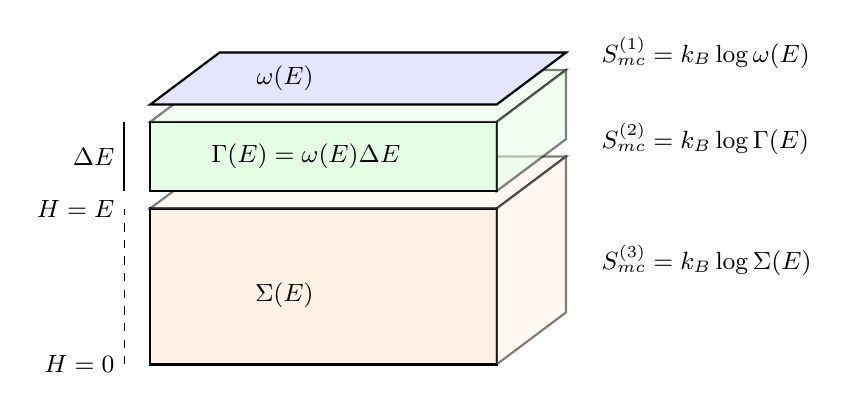
\begin{tikzpicture}[scale=1.1, every node/.style={font=\small}]

    % --- Parallelepipedo alto (da H=0 a H=E) ---
    \draw[thick, fill=orange!10] (-2,0.2) -- (2,0.2) -- (2,2.0) -- (-2,2.0) -- cycle;
    % parte posteriore vista dall’alto
    \draw[thick, fill=orange!10, opacity=0.5]
    (-2,2.0) -- (-1.2,2.6) -- (2.8,2.6) -- (2,2.0) -- cycle;
    \draw[thick, fill=orange!10, opacity=0.5]
    (2,0.2) -- (2,2.0) -- (2.8,2.6) -- (2.8,0.8) -- cycle;

    % --- Parallelepipedo basso (Delta E) ---
    \draw[thick, fill=green!10] (-2,2.2) -- (2,2.2) -- (2,3.0) -- (-2,3.0) -- cycle;
    % parte posteriore vista dall’alto
    \draw[thick, fill=green!10, opacity=0.5]
    (-2,3.0) -- (-1.2,3.6) -- (2.8,3.6) -- (2,3.0) -- cycle;
    \draw[thick, fill=green!10, opacity=0.5]
    (2,2.2) -- (2,3.0) -- (2.8,3.6) -- (2.8,2.8) -- cycle;

    % --- Rettangolo (in alto) ---
    \draw[thick, fill=blue!10]
    (-2,3.2) -- (-1.2,3.8) -- (2.8,3.8) -- (2,3.2) -- cycle;


    % Quotes
    \draw[dashed] (-2.3,0.2) -- (-2.3,2.0);
    \node[left] at (-2.3,0.2) {$H=0$};
    \node[left] at (-2.3,2.0) {$H=E$};

    \draw[thick] (-2.3,2.2) -- (-2.3,3.0);
    \node[left] at (-2.3,2.6) {$\Delta E$};

    \node[left] at (0.0,3.5) {$\omega(E)$};
    \node[left] at (1.0,2.6) {$\Gamma(E) = \omega(E)\Delta E$};
    \node[left] at (0.0,1.0) {$\Sigma(E)$};

    \node[right] at (3.1,3.8) {\(S_{mc}^{(1)}=k_B \log \omega(E)\)};
    \node[right] at (3.1,2.8) {\(S_{mc}^{(2)}=k_B \log \Gamma(E)\)};
    \node[right] at (3.1,1.4) {\(S_{mc}^{(3)}=k_B \log \Sigma(E)\)};

  \end{tikzpicture}

\end{figure}

By exploiting the relations between \(\omega(E)\), \(\Gamma(E)\) and \(\Sigma(E)\), one can equivalently write:
\[
  s_{mc} = k_B \lim_{td} \frac{\log \omega(E)}{N}
  = k_B \lim_{td} \frac{\log \Gamma(E)}{N}
  = k_B \lim_{td} \frac{\log \Sigma(E)}{N}
  = s_{th}.
\]
This identity is formally always true, although its physical realization can be explicitly verified only in specific models, such as the ideal gas. Thus we found that in the thermodynamic limit for the microcanonical ensemble there is a uniquely defined entropy.

At equilibrium, the properties of entropy satisfy the following key principles:
\begin{itemize}
  \item \textbf{Additivity:} For two independent subsystems, entropy is additive:
        \[
          S_{mc}^{(\text{tot})} = S_{mc}^{(1)} + S_{mc}^{(2)}.
        \]
        \begin{proof}
          Consider two independent subsystems with energies \(E_1\) and \(E_2\), such that the total energy is conserved: \(E = E_1 + E_2\). The two subsystems are independent:
          \[
            \mathcal{S}_1 : \begin{dcases}
              \mathcal{H}_1(q_i^{(1)}, p_i^{(1)}) = E_1, \quad (q_i^{(1)}, p_i^{(1)}) \in \mathcal{M}_1, \\
              \omega_1(E_1) = \int_{S_{\mathcal{H}_1=E_1}} \mathrm{d}  S_{\mathcal{H}_1} \implies S_{mc}^{(1)} = k_B \log \omega_1(E_1),
            \end{dcases}
          \]
          and the same applies to the second subsystem \(\mathcal{S}_2\) such that \(\mathcal{M} = \mathcal{M}_1 \times \mathcal{M}_2\). The total system \(\mathcal{S} = \mathcal{S}_1 + \mathcal{S}_2\) has a total density of states given by
          \[
            \omega(E) = \int_{\mathcal{M}} \d{\Omega} \delta(\mathcal{H} - E) = \int_{\mathcal{M}_1} \int_{\mathcal{M}_2} \d{\Omega_1} \d{\Omega_2} \, \delta(\mathcal{H}_1 + \mathcal{H}_2 - E).
          \]
          This integral can be decomposed by introducing an integral over the energy partition:
          \[
            \omega(E) = \int \d{\mathcal{H}_1} \int \d{\mathcal{H}_2} \int \d{S_{\mathcal{H}_1}} \int \d{S_{\mathcal{H}_2}} \delta(\mathcal{H}_2 - (E - \mathcal{H}_1)) = \int_0^E \d{\mathcal{H}_1} \, \omega_1(\mathcal{H}_1) \, \omega_2(E - \mathcal{H}_1).
          \]
          This quantity can be bounded above by the product of the densities of states of the subsystems, evaluated at the most probable energy partition (i.e. the one that maximizes the product) and multiplied by the total energy \(E\) (the upper bound of the integral):
          \[
            \omega(E) \leq E \, \omega_1(E_1^*) \, \omega_2(E_2^*),
          \]
          where \(E_1^*\) is the value that maximizes the product \(\omega_1(E_1) \omega_2(E - E_1)\), and \(E_2^* = E - E_1^*\).
          For a sufficiently small energy resolution \(\Delta E\), we can write the following bounds:
          \[
            \Delta E \, \omega_1(E_1^*) \, \omega_2(E_2^*) \leq \omega(E) \leq E \, \omega_1(E_1^*) \, \omega_2(E_2^*),
          \]
          Multiplying both sides by \(\Delta E\), we obtain:
          \[
            (\Delta E)^2 \, \omega_1(E_1^*) \, \omega_2(E_2^*) \leq \Delta E \, \omega(E) \leq E \, \Delta E \, \omega_1(E_1^*) \, \omega_2(E_2^*).
          \]
          Defining \(\Gamma(E) = \Delta E \, \omega(E)\) as the number of microstates in the energy shell \([E, E + \Delta E]\), we get:
          \[
            \Gamma_1(E_1^*) \, \Gamma_2(E_2^*) \leq \Gamma(E) \leq \frac{E}{\Delta E} \, \Gamma_1(E_1^*) \, \Gamma_2(E_2^*).
          \]
          To reconstruct the entropy, we take the logarithm of the inequality and multiply by Boltzmann's constant \(k_B\):\footnote{The logarithm is a monotonic function, so the inequality signs are preserved.}
          \[
            S_1(E_1^*) + S_2(E_2^*) \leq S(E) \leq S_1(E_1^*) + S_2(E_2^*) + k_B \log\left( \frac{E}{\Delta E} \right).
          \]
          Now we consider the thermodynamic limit, dividing by the total number of degrees of freedom \(N\) and taking \(N \to \infty\):
          \[
            \frac{S_1(E_1^*) + S_2(E_2^*)}{N} \leq \frac{S(E)}{N} \leq \frac{S_1(E_1^*) + S_2(E_2^*)}{N} + \frac{k_B \log\left( \frac{E}{\Delta E} \right)}{N}.
          \]
          Since the logarithmic correction vanishes in the thermodynamic limit (because \(\log\) grows sublinearly with \(N\)), we obtain:
          \[
            s_1(E_1^*) + s_2(E_2^*) \leq s(E) \leq s_1(E_1^*) + s_2(E_2^*),
          \]
          which implies:
          \[
            S_{mc}^{(\text{tot})} = S_{mc}^{(1)} + S_{mc}^{(2)}.
          \]
        \end{proof}
        \begin{remark}
          This property of entropy emerges in the thermodynamic limit at equilibrium, where the energies \(E_1^*\) and \(E_2^*\) are those that maximize the product of the densities of states of the two subsystems. This reflects the fact that the equilibrium configuration is the most probable one, corresponding to the maximum number of accessible microstates.
        \end{remark}

  \item \textbf{Equivalence with thermodynamic entropy:} In the thermodynamic limit,
        \[
          S_{mc} = S_{th},
        \]
        where \(S_{th}\) denotes the entropy defined by macroscopic thermodynamics.
        \begin{proof}
          Since \(\Gamma_1(E_1)\Gamma_2(E_2) = (\Delta E)^2 \, \omega_1(E_1)\omega_2(E_2)\), we can take its variation at the maximum point \((E_1^*,E_2^*)\), which must vanish at equilibrium:
          \[
            \delta \left\{ \Gamma_1(E_1)\Gamma_2(E_2) \right\}_{(E_1^*,E_2^*)} = 0 = \frac{\partial \Gamma_1(E_1)}{\partial E_1} \Bigg|_{E_1^*} \Delta E_1 \Gamma_2(E_2^*) + \Gamma_1(E_1^*) \frac{\partial \Gamma_2(E_2)}{\partial E_2} \Bigg|_{E_2^*} \Delta E_2.
          \]
          Since the total energy is conserved, we have \(\Delta E = \Delta E_1 + \Delta E_2 = 0\), which implies \(\Delta E_1 = -\Delta E_2\). Substituting this, we obtain:
          \[
            \frac{1}{\Gamma_1(E_1^*)} \frac{\partial \Gamma_1(E_1)}{\partial E_1} \Bigg|_{E_1^*} = \frac{1}{\Gamma_2(E_2^*)} \frac{\partial \Gamma_2(E_2)}{\partial E_2} \Bigg|_{E_2^*},
          \]
          which corresponds to the equality of logarithmic derivatives. Recalling the definition of microcanonical entropy, we can rewrite this as:
          \[
            \frac{\partial S_{mc}^{(1)}}{\partial E_1} \Bigg|_{E_1^*} = \frac{\partial S_{mc}^{(2)}}{\partial E_2} \Bigg|_{E_2^*}.
          \]
          This condition is equivalent to the thermodynamic equilibrium condition:
          \[
            \frac{\partial S_{mc}^{(1)}}{\partial E_1} \Bigg|_{E_1^*} = \frac{\partial S_{mc}^{(2)}}{\partial E_2} \Bigg|_{E_2^*} = \frac{1}{T},
          \]
          which expresses the equality of temperatures at equilibrium. Therefore, we conclude that the microcanonical entropy \(S_{mc}\) coincides with the thermodynamic entropy \(S_{th}\) in the thermodynamic limit.
        \end{proof}
\end{itemize}


Finally, the microcanonical entropy can also be expressed in the form of Boltzmann’s universal formula, which relates entropy to the average of the logarithm of the distribution function:
\begin{proposition}[Boltzmann’s formula]
  For the microcanonical ensemble one has
  \begin{equation}
    s_{mc} = -k_B \lim_{td} \frac{1}{N} \, \langle \log \rho_{mc} \rangle_{mc} = -k_B \lim_{td} \frac{1}{N} \int d\Omega \, \rho_{mc} \log \rho_{mc}.
    \label{eq:boltzmann_formula}
  \end{equation}
\end{proposition}
This shows the direct connection between Boltzmann’s statistical definition of entropy and the Gibbs–Shannon entropy of probability distributions, when restricted to the microcanonical setting.

\section{Perfect Gas}

As an explicit example of the microcanonical formalism, let us consider a gas of \(N\) non-relativistic and non-interacting monoatomic particles in three spatial dimensions. This is the paradigmatic system used to test the consistency of statistical mechanics with the laws of thermodynamics.

The phase space of the system is
\[
  \mathcal{M} = V^N \times \mathbb{R}^{3N} = \left\{ \{ (q_i, p_i) \}_{i=1}^N \; : \; q_i \in V, \, p_i \in \mathbb{R}^3 \right\},
\]
where each particle can move freely inside the container of volume \(V\), and the momentum space is unbounded.
The Hamiltonian is purely kinetic:
\[
  \mathcal{H}(q_i, p_i) = \sum_{i=1}^N \frac{p_i^2}{2m}, \qquad p_i = (p_i^x, p_i^y, p_i^z).
\]

\subsubsection{Volume and density of states}
The accessible phase space volume at fixed energy \(E\) can be computed explicitly as the integral over the phase space constrained by the energy shell,\footnote{The integral over space will give the volume to the power of \(N\), while for the integral over momenta one can go to spherical coordinates and use the volume of a \(3N\)-dimensional sphere: \(\frac{\pi^{d/2}}{\Gamma(d/2 + 1)}R^d\).} yielding
\[
  \Sigma(E) = \frac{2}{3} \left( \frac{V}{h^3} \right)^N \frac{(2\pi mE)^{3N/2}}{N \, \Gamma(3N/2)}.
\]
From this, the density of states follows:
\[
  \omega(E) = \frac{\partial \Sigma(E)}{\partial E} = \frac{3N}{2E} \, \Sigma(E),
  \qquad
  \Gamma(E) = \frac{3N}{2E} \, \Sigma(E)\,\Delta E.
\]
Hence, in the thermodynamic limit,
\[
  \lim_{td} \frac{\log \Sigma(E)}{N} = \lim_{td} \frac{\log \omega(E)}{N} = \lim_{td} \frac{\log \Gamma(E)}{N}.
\]

\subsubsection{Entropy for distinguishable particles}
For distinguishable particles, the entropy can be computed in the thermodynamic limit as \(S = k_B \log(\Sigma(E))\), remembering that
\[
  \Gamma(x + 1) = x! = x \, \Gamma(x) \quad \Rightarrow \quad \Gamma(1/2) = \sqrt{\pi}.
\]
Thus, using Stirling's approximation for large \(N\), \(\log N! \approx N \log N - N\), one obtains
\[
  S = \frac{3}{2} N k_B + N k_B \log \left[ V \left( \frac{4\pi mE}{3Nh^2} \right)^{3/2} \right].
\]
From this expression one recovers the standard thermodynamic relations:
\begin{align*}
  \frac{1}{T} & = \left.\frac{\partial S}{\partial E}\right|_{V,N} \quad \Rightarrow \quad E = \frac{3}{2} N k_B T, \\[0.5em]
  \frac{p}{T} & = \left.\frac{\partial S}{\partial V}\right|_{E,N} \quad \Rightarrow \quad pV = N k_B T.
\end{align*}
However, this entropy is not extensive, as it grows faster than linearly with \(N\). Furthermore, we will interpret the result for the energy as the \textit{classical equipartition theorem}, assigning an average energy of \(\frac{1}{2} k_B T\) to each quadratic degree of freedom.

\subsubsection{Entropy for indistinguishable particles}
Correct extensivity is restored by taking into account the indistinguishability of identical particles, which introduces the Gibbs correction factor \(1/N!\).\footnote{This factor was naturally incorporated inside the measure of the phase space in \eqref{eq:dimensionless_measure_phase_space} in order to reach a rigorous treatment of the indistinguishable states (renormalizing accordingly) in the phase space.} The resulting entropy is
\[
  S = \frac{5}{2} N k_B + 3N k_B \log \left( \frac{d}{\lambda_T} \right),
\]
where
\[
  d^3 \equiv \frac{V}{N}, \qquad \lambda_T \equiv \sqrt{\frac{h^2}{2\pi m k_B T}}
\]
is the \textit{thermal wavelength}. This expression is extensive and coincides with the classical Sackur--Tetrode formula.

\subsubsection{Limits of validity}
The microcanonical entropy becomes negative for sufficiently low temperatures,
\[
  T < T^* \equiv \frac{e^{-5/3} h^2}{2\pi m k_B d^2},
\]
corresponding to densities such that \(d \lesssim \lambda_T\). This signals the breakdown of the classical approximation, and the necessity to include quantum statistics (Bose–Einstein or Fermi–Dirac) in the description of the gas.
